\documentclass{standalone}

\usepackage{pgfplots,tikz,amsmath}
\begin{document}
        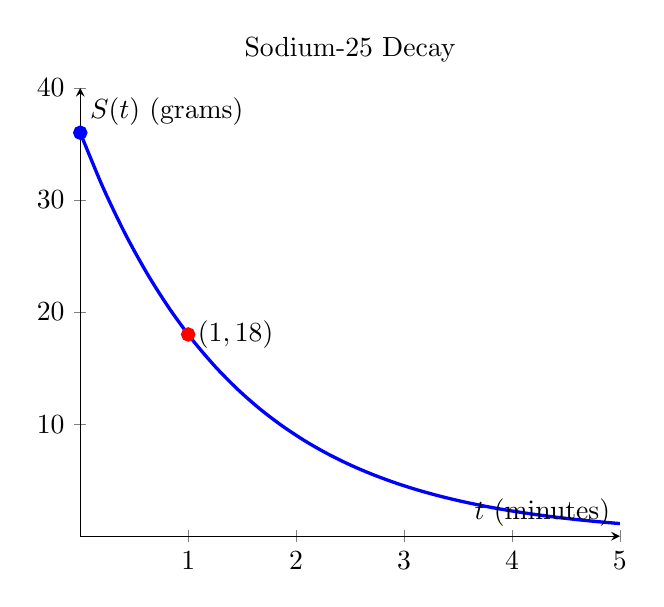
\begin{tikzpicture}
            \begin{axis}[axis lines=center, xlabel={$t$ (minutes)}, ylabel={$S(t)$
                (grams)}, xmin=0, xmax=5,ymin=0, ymax=40, domain=0:5, title={Sodium-25
                Decay}]
                \addplot[blue, very thick, smooth] {36*(0.5)^x};
                \addplot[mark=*,red,very thick] coordinates{(1,18)};
                \addplot[mark=*,blue,very thick] coordinates{(0,36)};
                \draw (axis cs:1,18) node[anchor=west]{$(1,18)$};
            \end{axis}
        \end{tikzpicture}
\end{document}
